% The placement matrix of the one-cube box, in Figure 1's orientation.
% Compile with pdfLaTeX.
\documentclass[tikz,border=3pt]{standalone}
\usepackage[T1]{fontenc}
\usepackage{lmodern,amsmath,amssymb}
\pdfinfoomitdate=1
\pdftrailerid{}
\pdfsuppressptexinfo=15
\pdfinfo{/Title (The tiling group of the one-cube box) /Author (twinheterodox)}

\definecolor{ink}{HTML}{223A41}
\definecolor{emptyedge}{HTML}{236866}
\definecolor{emptymark}{HTML}{E1F1EE}
\definecolor{cubeedge}{HTML}{99521D}
\definecolor{cubemark}{HTML}{FFF0D5}
\definecolor{floor}{HTML}{FAF2E3}
\definecolor{wall}{HTML}{EFF4F3}
\definecolor{rightwall}{HTML}{E4EEEB}
\definecolor{top}{HTML}{EBCB95}
\definecolor{sideleft}{HTML}{B8D1CD}
\definecolor{sideright}{HTML}{D3E5DF}

% Triangle i lies between rim vertices i and i+1, clockwise from the top.
\newcommand{\rim}[1]{({90-60*(#1)}:1)}
\newcommand{\drawtile}[2]{\filldraw[fill=#2,draw=ink,line width=.8pt]
  (0,0)--\rim{#1}--\rim{#1+1}--\rim{#1+2}--cycle;}
\newcommand{\markdiagonal}[3]{%
  \draw[#2,densely dotted,line width=.7pt] (0,0)--\rim{#1+1};
  \node[#3,minimum size=1.85mm] at ({90-60*(#1+1)}:.53) {};}
\newcommand{\trinames}{%
  \foreach \i/\n in {0/x,1/A,2/y,3/B,4/z,5/C}
    \node[inner sep=0pt] at ({60-60*\i}:.64) {\(\n\)};}

\begin{document}
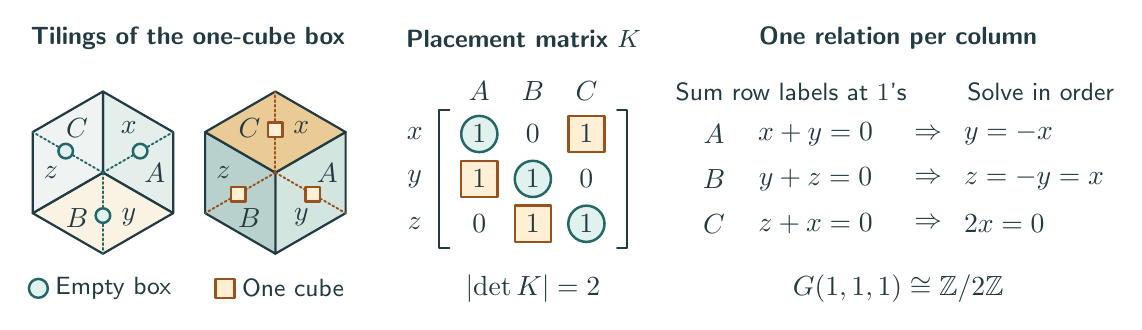
\begin{tikzpicture}[text=ink,font=\normalsize,line join=round,line cap=round,
  heading/.style={font=\sffamily\small\bfseries,inner sep=0pt},
  key/.style={font=\sffamily\small,inner sep=0pt},
  empty mark/.style={circle,draw=emptyedge,fill=emptymark,inner sep=0pt,line width=.9pt},
  cube mark/.style={rectangle,draw=cubeedge,fill=cubemark,inner sep=0pt,line width=.9pt},
  entry/.style={inner sep=0pt,minimum size=4.6mm},
  formula/.style={inner sep=0pt}]
  \node[heading] at (2.08,1.82) {Tilings of the one-cube box};
  \node[heading] at (6.34,1.82) {Placement matrix \(K\)};
  \node[heading] at (11.10,1.82) {One relation per column};

  % Each symbol sits on the short diagonal of exactly one lozenge.
  \begin{scope}[shift={(1.00,.12)},scale=1.03]
    \drawtile{0}{rightwall}\drawtile{2}{floor}\drawtile{4}{wall}
    \foreach \i in {0,2,4} {\markdiagonal{\i}{emptyedge}{empty mark}}
    \trinames
  \end{scope}
  \begin{scope}[shift={(3.19,.12)},scale=1.03]
    \drawtile{1}{sideright}\drawtile{3}{sideleft}\drawtile{5}{top}
    \foreach \i in {1,3,5} {\markdiagonal{\i}{cubeedge}{cube mark}}
    \trinames
  \end{scope}
  \node[empty mark,minimum size=2.4mm] at (.18,-1.35) {};
  \node[key,anchor=west] at (.39,-1.35) {Empty box};
  \node[cube mark,minimum size=2.4mm] at (2.55,-1.35) {};
  \node[key,anchor=west] at (2.76,-1.35) {One cube};

  % One 1 per tile; the three marks of either shape form a full matching.
  \foreach \X/\col in {5.78/A,6.46/B,7.14/C} \node at (\X,1.15) {\(\col\)};
  \foreach \Y/\row in {.61/x,.04/y,-.53/z} \node at (4.96,\Y) {\(\row\)};
  \draw[ink,line width=.75pt] (5.40,.92)--(5.27,.92)--(5.27,-.84)--(5.40,-.84);
  \draw[ink,line width=.75pt] (7.53,.92)--(7.66,.92)--(7.66,-.84)--(7.53,-.84);
  \foreach \X/\Y in {5.78/.61,6.46/.04,7.14/-.53}
    \node[empty mark,entry] at (\X,\Y) {\(1\)};
  \foreach \X/\Y in {7.14/.61,5.78/.04,6.46/-.53}
    \node[cube mark,entry] at (\X,\Y) {\(1\)};
  \foreach \X/\Y in {6.46/.61,7.14/.04,5.78/-.53}
    \node[entry] at (\X,\Y) {\(0\)};
  \node[formula] at (6.46,-1.35) {\(\lvert\det K\rvert=2\)};

  \node[key] at (9.74,1.15) {Sum row labels at \(1\)'s};
  \node[key] at (12.91,1.15) {Solve in order};
  \foreach \Y/\col/\rel/\result in {
      .61/A/{x+y=0}/{y=-x},
      .04/B/{y+z=0}/{z=-y=x},
      -.53/C/{z+x=0}/{2x=0}} {
    \node[formula] at (8.76,\Y) {\(\col\)};
    \node[formula] at (10.05,\Y) {\(\rel\)};
    \node[formula] at (11.48,\Y) {\(\Rightarrow\)};
    \node[formula,anchor=west] at (11.93,\Y) {\(\result\)};
  }
  \node[formula] at (11.10,-1.35) {\(G(1,1,1)\cong\mathbb Z/2\mathbb Z\)};
\end{tikzpicture}
\end{document}
